\documentclass{article}
\usepackage{amsmath, amssymb}
\usepackage{tikz}
\usetikzlibrary{matrix, positioning, arrows.meta}

\begin{document}

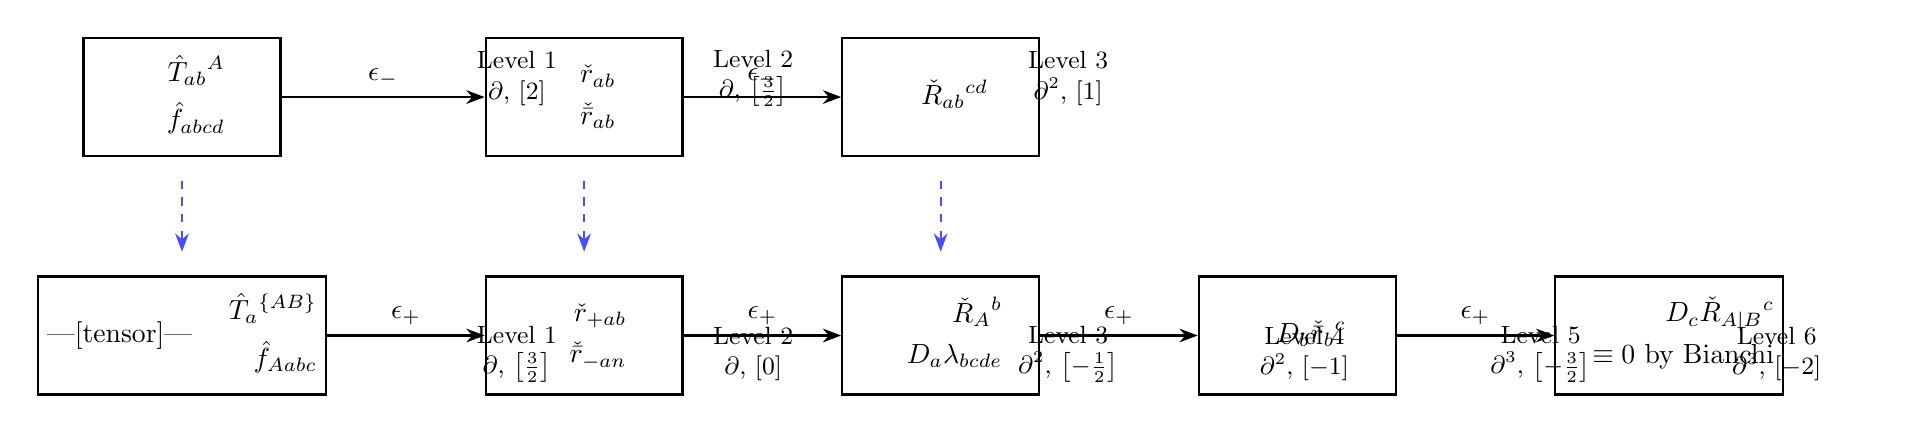
\begin{tikzpicture}[node distance=2cm, auto,
    tensor/.style={rectangle, draw, thick, minimum width=2.5cm, minimum height=1.5cm},
    arrow/.style={->, >=Stealth, thick},
    levellabel/.style={text width=3cm, align=center, font=\small},
    boost/.style={->, >=Stealth, thick, dashed, blue!70}
]

% Define positions for nodes
\matrix (m) [matrix of nodes, column sep=2cm, row sep=1.5cm, nodes={tensor}] {
    % Top row
    |[tensor]| {$\begin{aligned}
        &\hat{T}_{ab}{}^A \\
        &\hat{f}_{abcd}
    \end{aligned}$} &
    |[tensor]| {$\begin{aligned}
        &\check{r}_{ab} \\
        &\check{\bar{r}}_{ab}
    \end{aligned}$} &
    |[tensor]| {$\begin{aligned}
        &\check{R}_{ab}{}^{cd} \\
    \end{aligned}$} \\
    
    % Bottom row
    |[tensor]| {$\begin{aligned}
        &\hat{T}_a{}^{\{AB\}} \\
        &\hat{f}_{Aabc}
    \end{aligned}$} &
    |[tensor]| {$\begin{aligned}
        &\check{r}_{+ab} \\
        &\check{\bar{r}}_{-an}
    \end{aligned}$} &
    |[tensor]| {$\begin{aligned}
        &\check{R}_A{}^b \\
        &D_a\lambda_{bcde}
    \end{aligned}$} &
    |[tensor]| {$\begin{aligned}
        &D_b\check{\bar{r}}{}_b{}^c \\
    \end{aligned}$} &
    |[tensor]| {$\begin{aligned}
        &D_c\check{R}_{A|B}{}^c \\
        &\equiv 0 \text{ by } \text{Bianchi}
    \end{aligned}$} \\
};

% Add level labels
\node[levellabel] at (-5, 1.75) {Level 1 \\ $\partial$, $[2]$};
\node[levellabel] at (-2, 1.75) {Level 2 \\ $\partial$, $\left[\frac{3}{2}\right]$};
\node[levellabel] at (2, 1.75) {Level 3 \\ $\partial^2$, $[1]$};
\node[levellabel] at (-5, -1.75) {Level 1 \\ $\partial$, $\left[\frac{3}{2}\right]$};
\node[levellabel] at (-2, -1.75) {Level 2 \\ $\partial$, $[0]$};
\node[levellabel] at (2, -1.75) {Level 3 \\ $\partial^2$, $\left[-\frac{1}{2}\right]$};
\node[levellabel] at (5, -1.75) {Level 4 \\ $\partial^2$, $[-1]$};
\node[levellabel] at (8, -1.75) {Level 5 \\ $\partial^3$, $\left[-\frac{3}{2}\right]$};
\node[levellabel] at (11, -1.75) {Level 6 \\ $\partial^3$, $[-2]$};

% Draw horizontal arrows
\draw[arrow] (m-1-1) -- node[above] {$\epsilon_-$} (m-1-2);
\draw[arrow] (m-1-2) -- node[above] {$\epsilon_-$} (m-1-3);

\draw[arrow] (m-2-1) -- node[above] {$\epsilon_+$} (m-2-2);
\draw[arrow] (m-2-2) -- node[above] {$\epsilon_+$} (m-2-3);
\draw[arrow] (m-2-3) -- node[above] {$\epsilon_+$} (m-2-4);
\draw[arrow] (m-2-4) -- node[above] {$\epsilon_+$} (m-2-5);

% Draw vertical arrows (boosts)
\draw[boost] ([yshift=-0.3cm]m-1-1.south) -- node[right] {} ([yshift=0.3cm]m-2-1.north);
\draw[boost] ([yshift=-0.3cm]m-1-2.south) -- node[right] {} ([yshift=0.3cm]m-2-2.north);
\draw[boost] ([yshift=-0.3cm]m-1-3.south) -- node[right] {} ([yshift=0.3cm]m-2-3.north);

\end{tikzpicture}

\end{document}